\documentclass[a4paper,12pt]{article}
\usepackage[latin1]{inputenc}
\usepackage[spanish]{babel}
\usepackage{bm}
\usepackage{graphicx}
\usepackage{amsmath}
\setlength{\textheight}{235mm}
\setlength{\textwidth}{168mm}
\setlength{\oddsidemargin}{0pt}
\pagestyle{empty}
\begin{document}
\mbox{}\vspace*{-45mm}

{\centering
{\small\sc Escuela T�cnica Superior de Ingenieros de Caminos, Canales y
Puertos (Madrid)}\\*[4mm]
{\Large\bf M�todo de los Elementos Finitos (Curso 20-21)}\\*[4mm]
EXAMEN FINAL ORDINARIO (8 de febrero de 2021) \\*[4mm]
}

\vspace{3mm}

%%%%%
\noindent
Tiempo: 60 minutos
\noindent
\paragraph{Ejercicio 1.} La chapa de la figura tiene un coeficiente
de conductividad t�rmica $k=60$ W/(m$\cdot$K).
El borde inferior horizontal est� a una temperatura de $173$ $^{\circ}$ K
y el borde vertical de la izquierda a una
temperatura de $473$ $^{\circ}$ K. Los dem�s bordes est�n t�rmicamente
aislados.

Se pide:
\begin{enumerate}
\item Hacer el modelo de elementos finitos correspondiente, y contestar a las
preguntas del cuestionario disponible en el sitio Moodle de la asignatura.
\item Cargar en el enlace correspondiente de Moodle el fichero {\tt FeapAAAA.eps} con los contornos de flujo en direcci�n $x$
\end{enumerate}
{\bf NOTAS:}
\begin{enumerate}
\item La malla se definir� con los dos bloques indicados en la figura, numerando
sus esquinas con el criterio que tambi�n viene indicado en dicha figura.
\item El bloque $1$ est� discretizado con $15$ elementos en direcci�n
$x$ y $30$ elementos en direcci�n $y$. El bloque $2$ tambi�n tiene una
discretizaci�n de $15 \times 30$ elementos. Todos los elementos son
cuadril�teros bilineales.
\end{enumerate}

\begin{center}
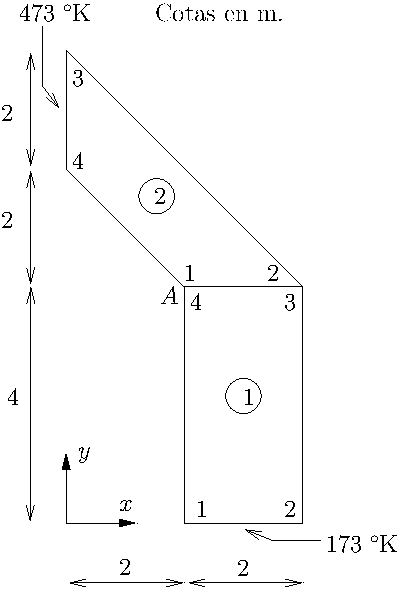
\includegraphics[width=0.4\textwidth]{ejer1.pdf}
\hspace{5mm}
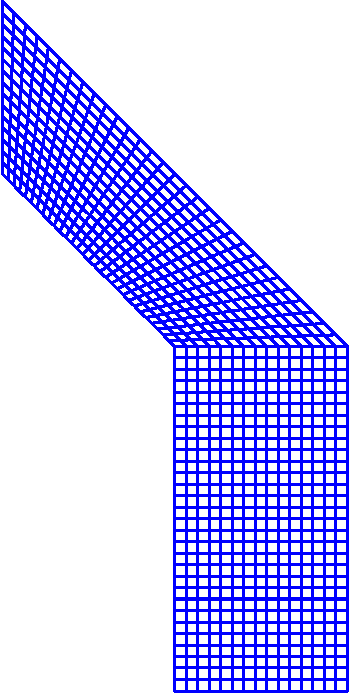
\includegraphics[width=0.25\textwidth]{malla.pdf}
\end{center}

\end{document}
